\documentclass[UTF8]{ctexart}
\usepackage[a4paper,left=3cm,right=3cm,top=2cm]{geometry}
\usepackage{amsmath}
\usepackage{enumitem}
\usepackage{float}
\usepackage{threeparttable}
\usepackage{caption}
\usepackage{multirow}
\usepackage{graphicx}

\setlength\lineskiplimit{5.25bp}
\setlength\lineskip{5.25bp}

\title{自由落体法测量重力加速度——实验报告}
\author{崔士强 PB22151743}
\date{\today}

\bibliographystyle{plain}

\begin{document}

\maketitle
\section{实验目的}
本实验利用自由落体测量重力加速度.
\section{实验原理}
由匀加速直线运动规律知
\[h=v_0t+\frac{1}{2}gt^2\]
\indent 两端同时除以$t$得
\[\overline{v}=v_0+\frac{1}{2}gt\]
\indent 可以看到一段时间内平均速度$\overline{v}$与经过的时间$t$具有线性关系,因此测量多组数据进行线性拟合可以求出重力加速度$g$
\section{实验仪器}
本实验使用光电门进行测量,实验仪器如下图所示
\begin{figure}[h]
    \centering
    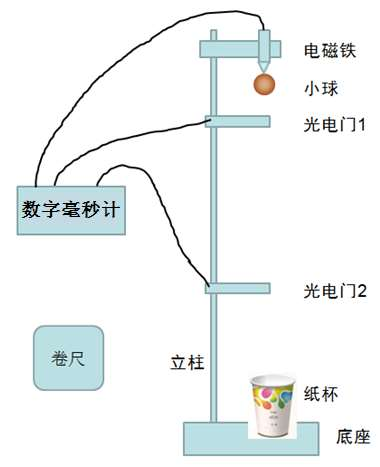
\includegraphics[scale=0.3]{p2.png}
    \caption{实验仪器}
\end{figure}

由于电磁铁断电时有剩磁,这里测量下落过程中经过两个光电门时间之差
\section{实验数据及处理}
实验数据见下表,原始数据记录照片见文档尾.
\begin{table}[H]
    \centering
    \begin{tabular}{cccc}
        \hline\hline
        \multicolumn{2}{c}{大球}&\multicolumn{2}{c}{小球}\\
        $\Delta h/cm$&$\Delta t/ms$&$\Delta h/cm$&$\Delta t/ms$\\
        \hline
        35&149.7&35&148.8\\
        40&165.8&40&164.7\\
        45&180.8&45&179.8\\
        50&195.4&50&194.4\\
        \hline\hline
    \end{tabular}
\end{table}
\begin{enumerate}
    \item [1).]大球的线性拟合数据:
    \begin{figure}[h]
        \centering
        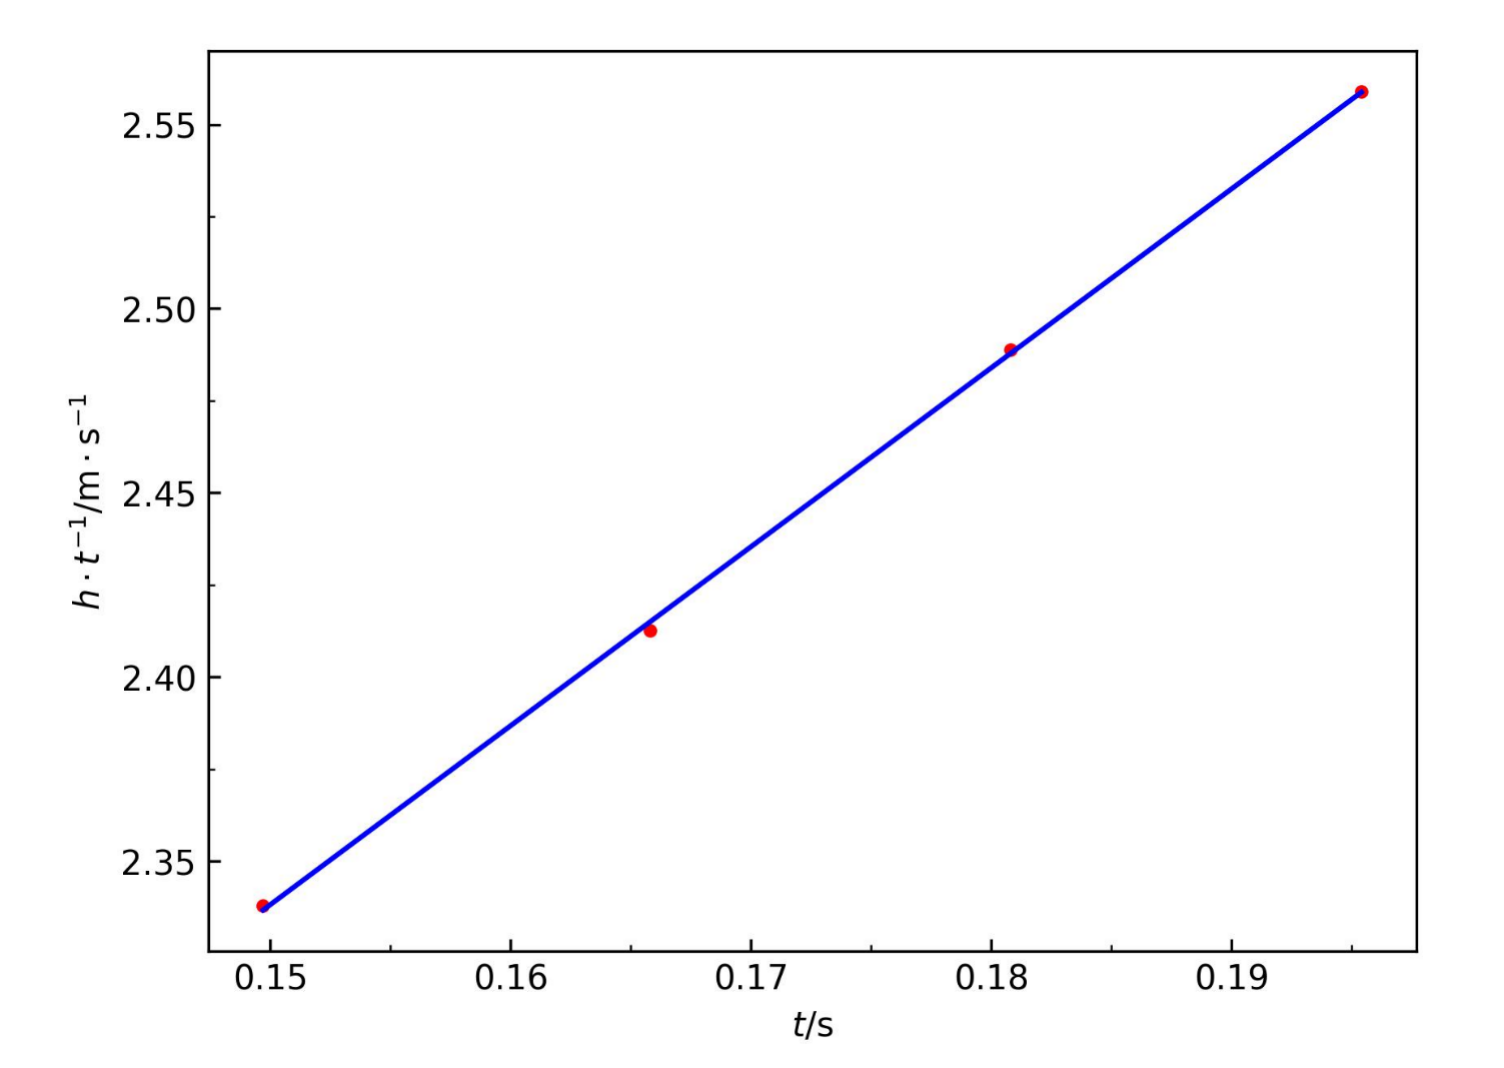
\includegraphics[scale=0.5]{big.png}
        \caption{大球下落平均速度与时间关系曲线}
    \end{figure}
    
    \noindent 斜率
    $$
    m=4.8569\,\mathrm{m/s^2}
    $$
    截距
    $$
    b=1.6097\,\mathrm{m/s}
    $$
    线性拟合的相关系数
    $$
    r=\frac{\overline{tv}-\overline{t}\cdot\overline{v}}{\sqrt{\left(\overline{t^2}-\overline{t}^2\right)\left(\overline{v^2}-\overline{v}^2\right)}}=0.9998414
    $$
    斜率标准差
    $$
    s_m=\lvert m\rvert\cdot\sqrt{\left(\frac{1}{r^2}-1\right)/(n-2)}=0.061174\,\mathrm{m/s^2}
    $$
    截距标准差
    $$
    s_b=s_m\cdot\sqrt{\overline{t^2}}=0.01063\,\mathrm{m/s}
    $$
    
    \noindent 重力加速度
    $$
    g=2 m=2\times 4.8569\,\mathrm{m/s^2}=9.7139\,\mathrm{m/s^2}
    $$
    \item [2).]小球的线性拟合数据:
    \begin{figure}[h]
        \centering
        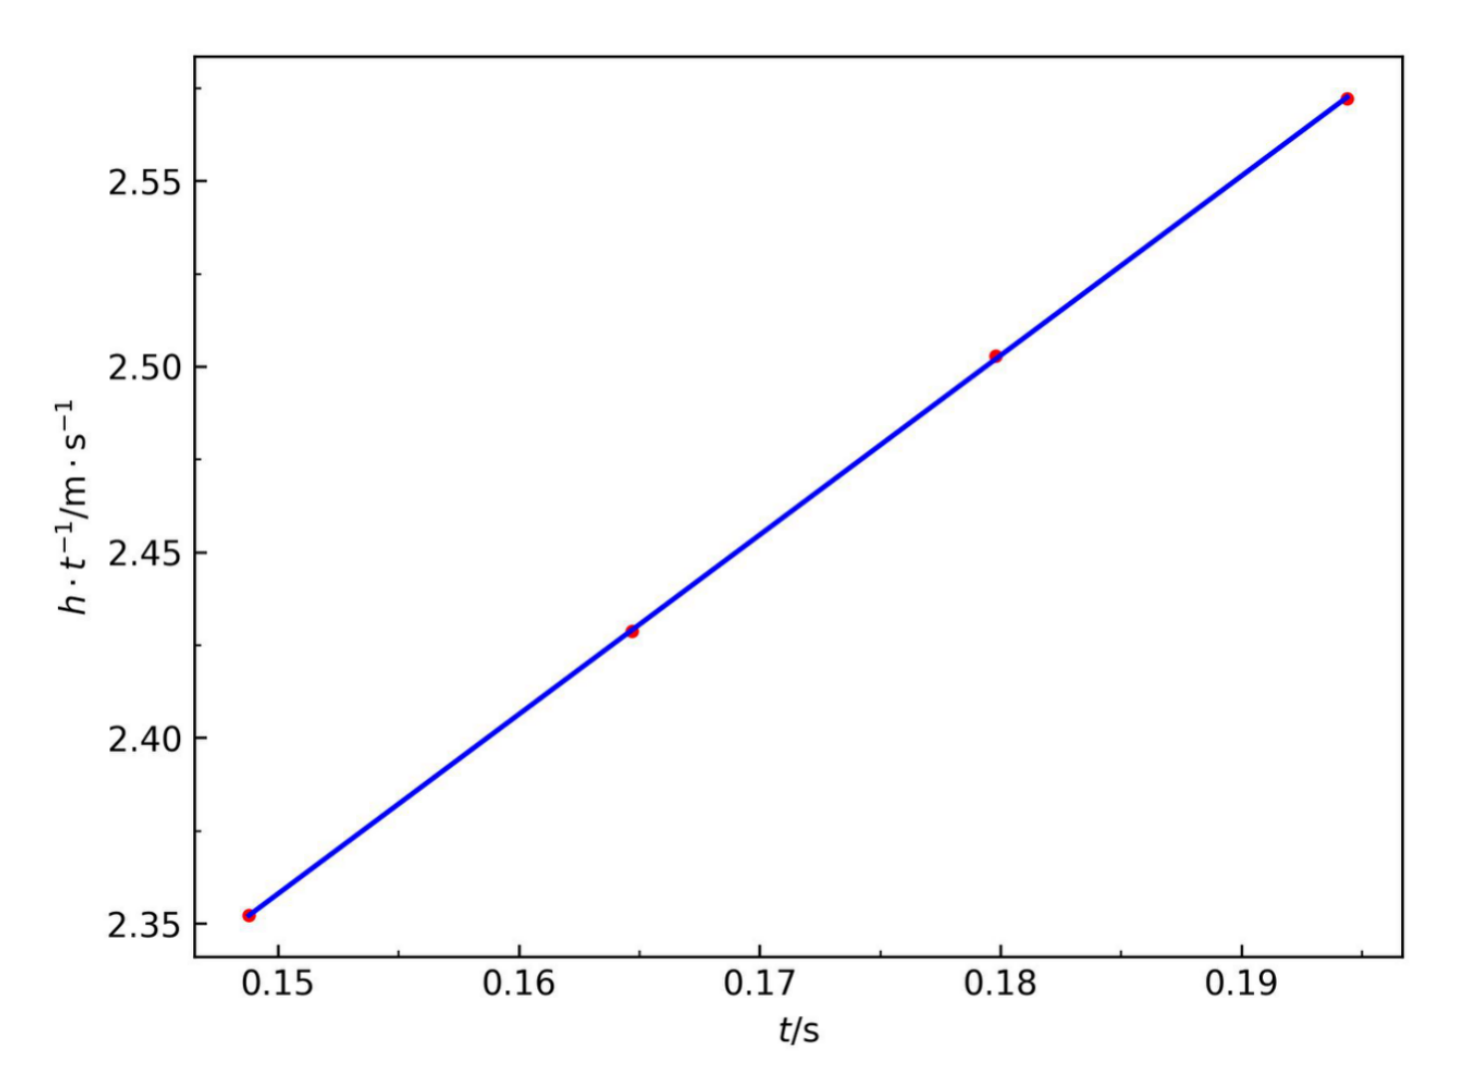
\includegraphics[scale=0.5]{small.png}
        \caption{小球下落平均速度与时间关系曲线}
    \end{figure}
    
    \noindent 斜率
    $$
    m=4.8305\,\mathrm{m/s^2}
    $$
    截距
    $$
    b=1.6334\,\mathrm{m/s}
    $$
    线性拟合的相关系数
    $$
    r=\frac{\overline{tv}-\overline{t}\cdot\overline{v}}{\sqrt{\left(\overline{t^2}-\overline{t}^2\right)\left(\overline{v^2}-\overline{v}^2\right)}}=0.99998093
    $$
    斜率标准差
    $$
    s_m=\lvert m\rvert\cdot\sqrt{\left(\frac{1}{r^2}-1\right)/(n-2)}=0.021093\,\mathrm{m/s^2}
    $$
    截距标准差
    $$
    s_b=s_m\cdot\sqrt{\overline{t^2}}=0.003644\,\mathrm{m/s}
    $$
    重力加速度
    $$
    g=2 m=2\times 4.8305\,\mathrm{m/s^2}=9.661\,\mathrm{m/s^2}
    $$
\end{enumerate}
\section{误差分析}
可以看到实验测得重力加速度值比预计值$g=9.7947m/s^2$偏小,且小球测得重力加速度值更小,推测原因有以下几点:
\begin{enumerate}
    \item [1).] 空气阻力对实验产生影响,且小球受这种影响更为显著;
    \item [2).] 两个光电门之间距离的测量值偏小.
\end{enumerate}
\section{思考题}
\begin{enumerate}
    \item 电磁铁断电时有剩磁,导致开始下落的时间难以测准,小球做匀加速直线运动的时间不准;
    \item 下落时间过长时空气阻力导致的影响积累,故第一个光电门应放置在靠近电磁铁的位置,第二个光电门根据所需高度差放置;
    \item 只用一个光电门,测量光电门到电磁铁的距离,多次改变光电门位置,对下落高度与时间的关系进行二次拟合,根据二次项系数得出重力加速度值,这种方法可以避开思考题1所提到的误差,原因是起始时间不影响二次项系数
\end{enumerate}
\section{原始数据记录}
\begin{figure}[h]
    \centering
    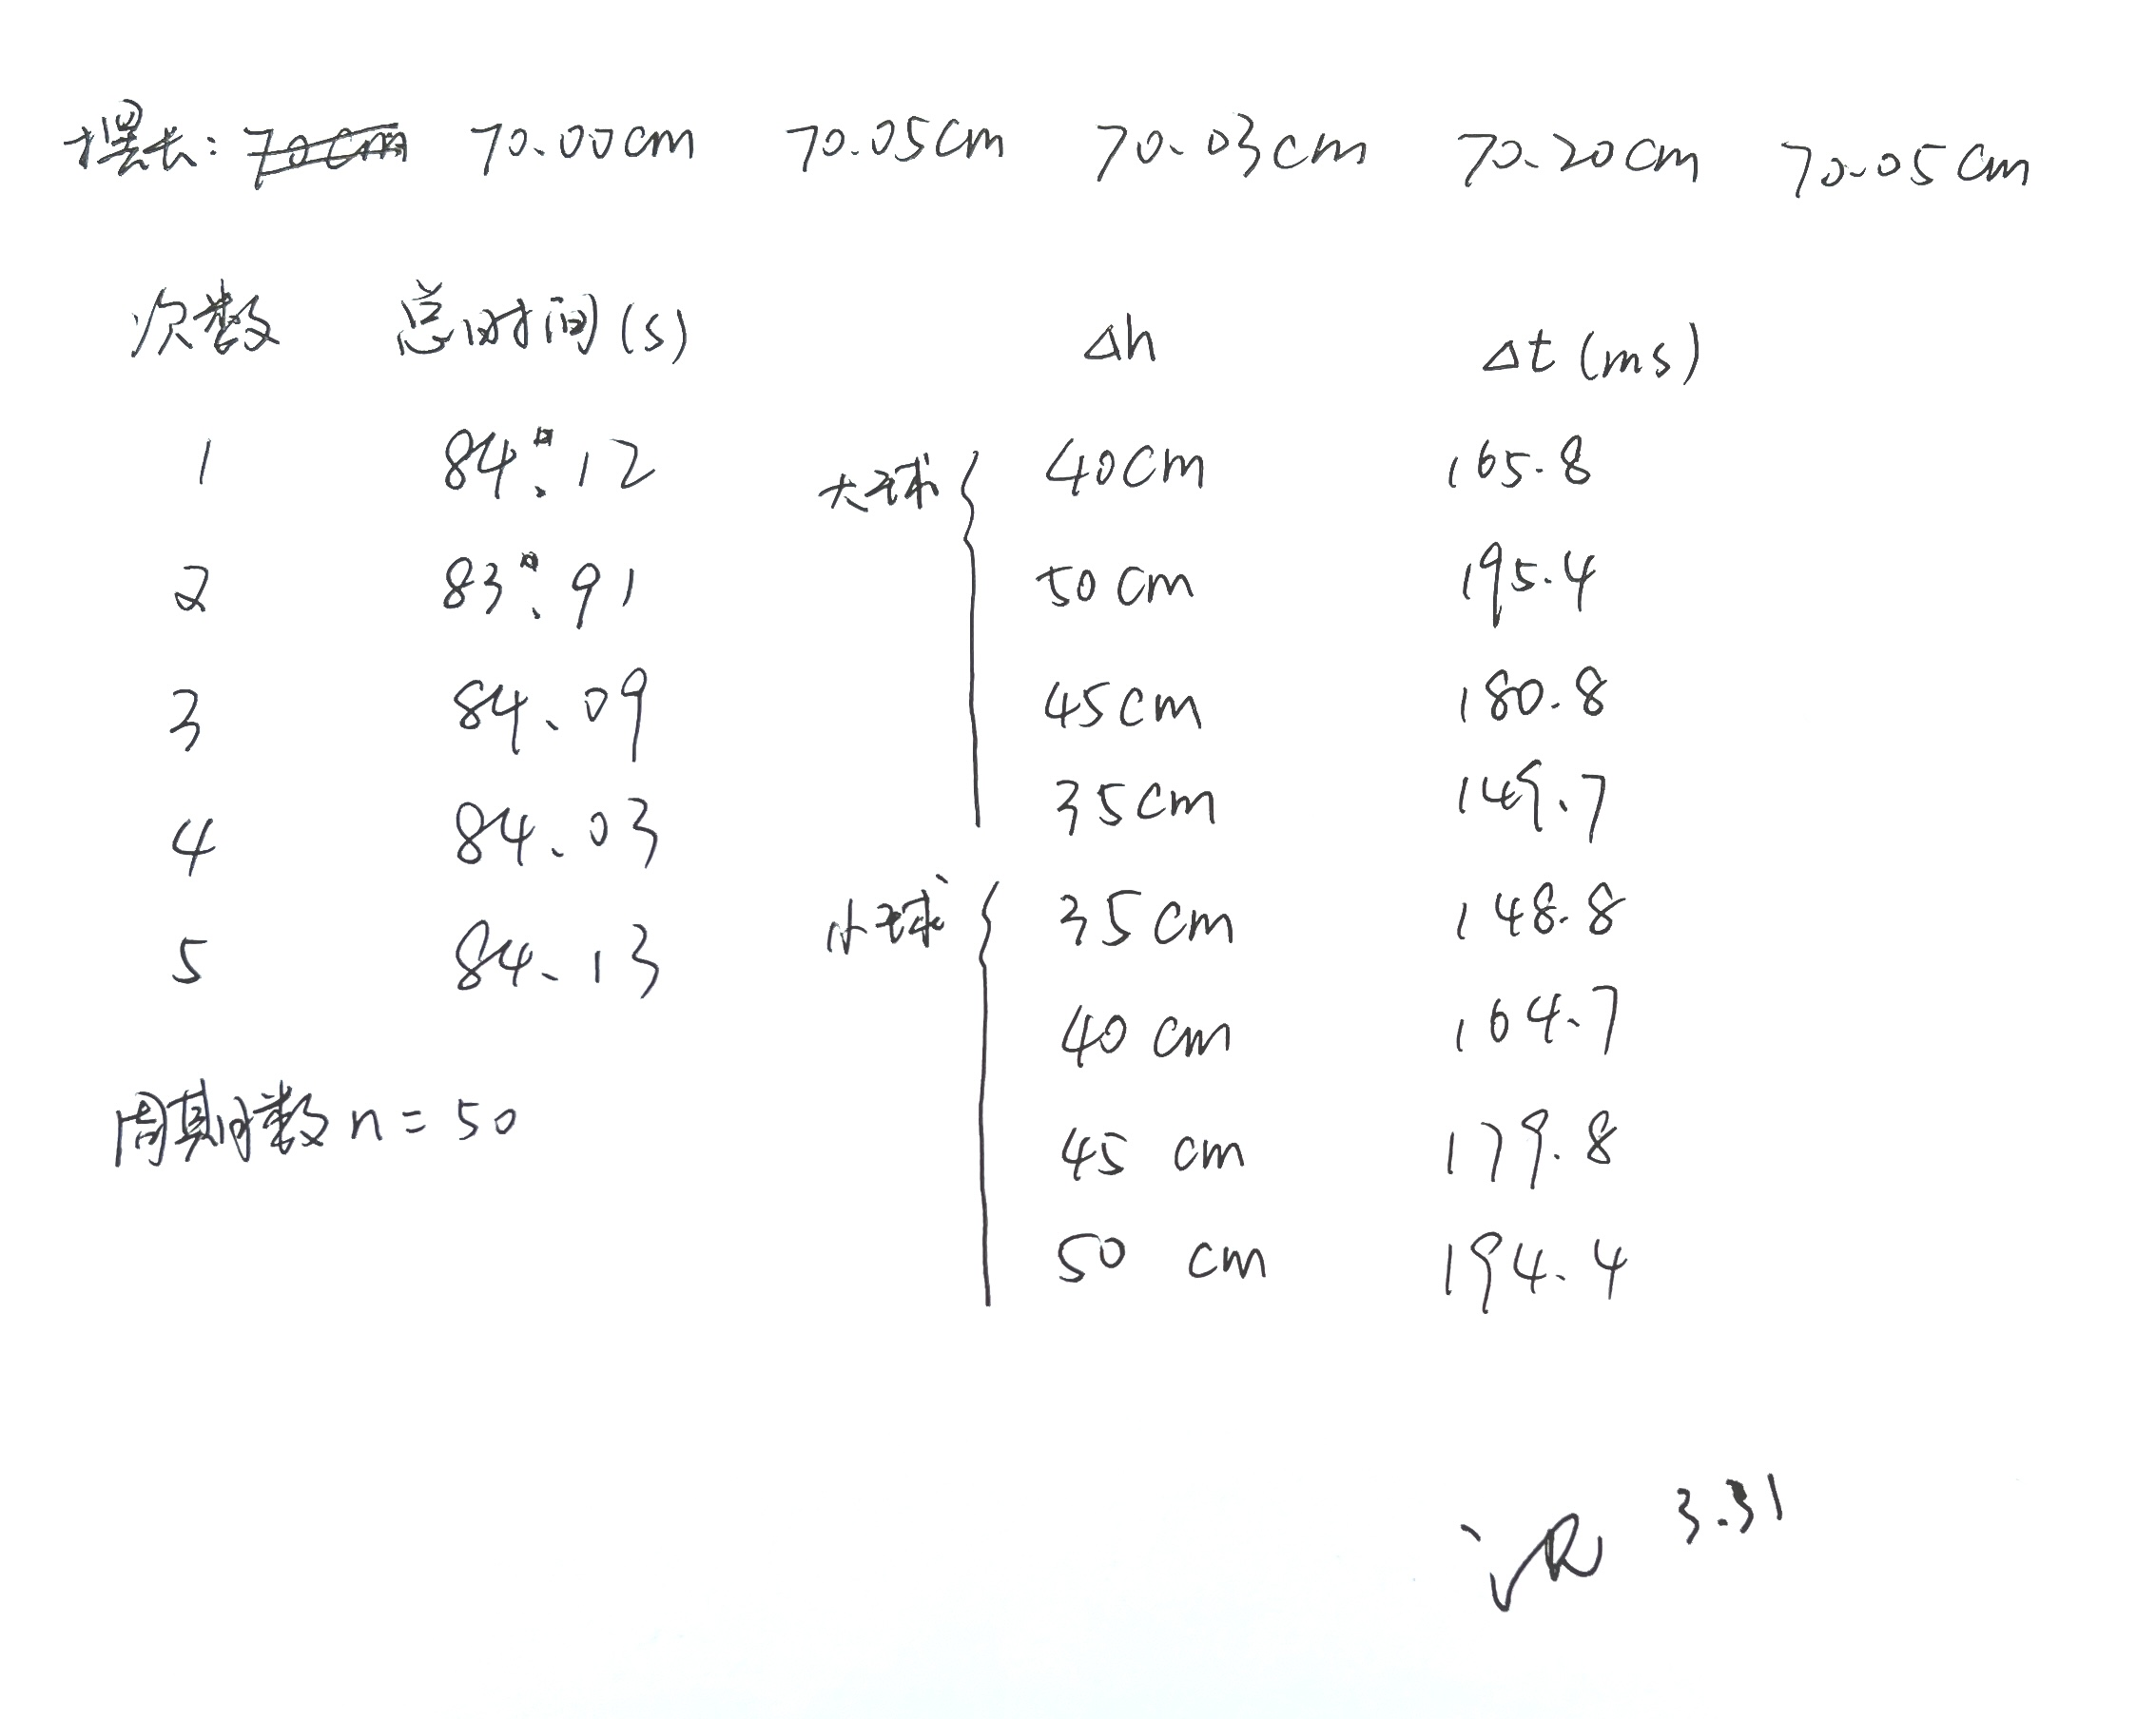
\includegraphics[scale=0.55]{data.png}
\end{figure}

\bibliography{math}

\end{document}